\section{3D displays}

\subsection{Volumetric Displays}
Volumetric displays \cite{1492264} are a promising technology that offers a captivating three-dimensional viewing experience. By emitting light for each voxel, or volume element, in a 3D space, these displays transcend the limitations of traditional 2D planes, providing a truly immersive 3D effect. This innovative approach enables the accurate representation of virtual 3D objects, including focal depth, motion parallax, and vergence, which refers to the rotation of a viewer's eye to fixate on the same point they are focusing on . Moreover, volumetric displays allow multiple users to view the same display from different angles, providing unique perspectives of the same object. 

\subsubsection{Swept Volume Displays}
Swept volume displays represent one category of volumetric displays. They employ a moving 2D display to create a 3D image. This is achieved by moving the 2D display through a 3D space and emitting light from the display at each point. Common techniques for achieving this includes using a rotating mirror, emitting screen typically an LED \cite{Gately:11}, or transparent surface that can be projected onto. There currently exist commercial products that implement this technology, Two examples can be seen in Fig~\ref{fig:swept-volume-displays}.

\begin{figureBox}[label={fig:swept-volume-displays}]{Two different types of swept volume display}
    \begin{minipage}[t]{0.48\textwidth}
      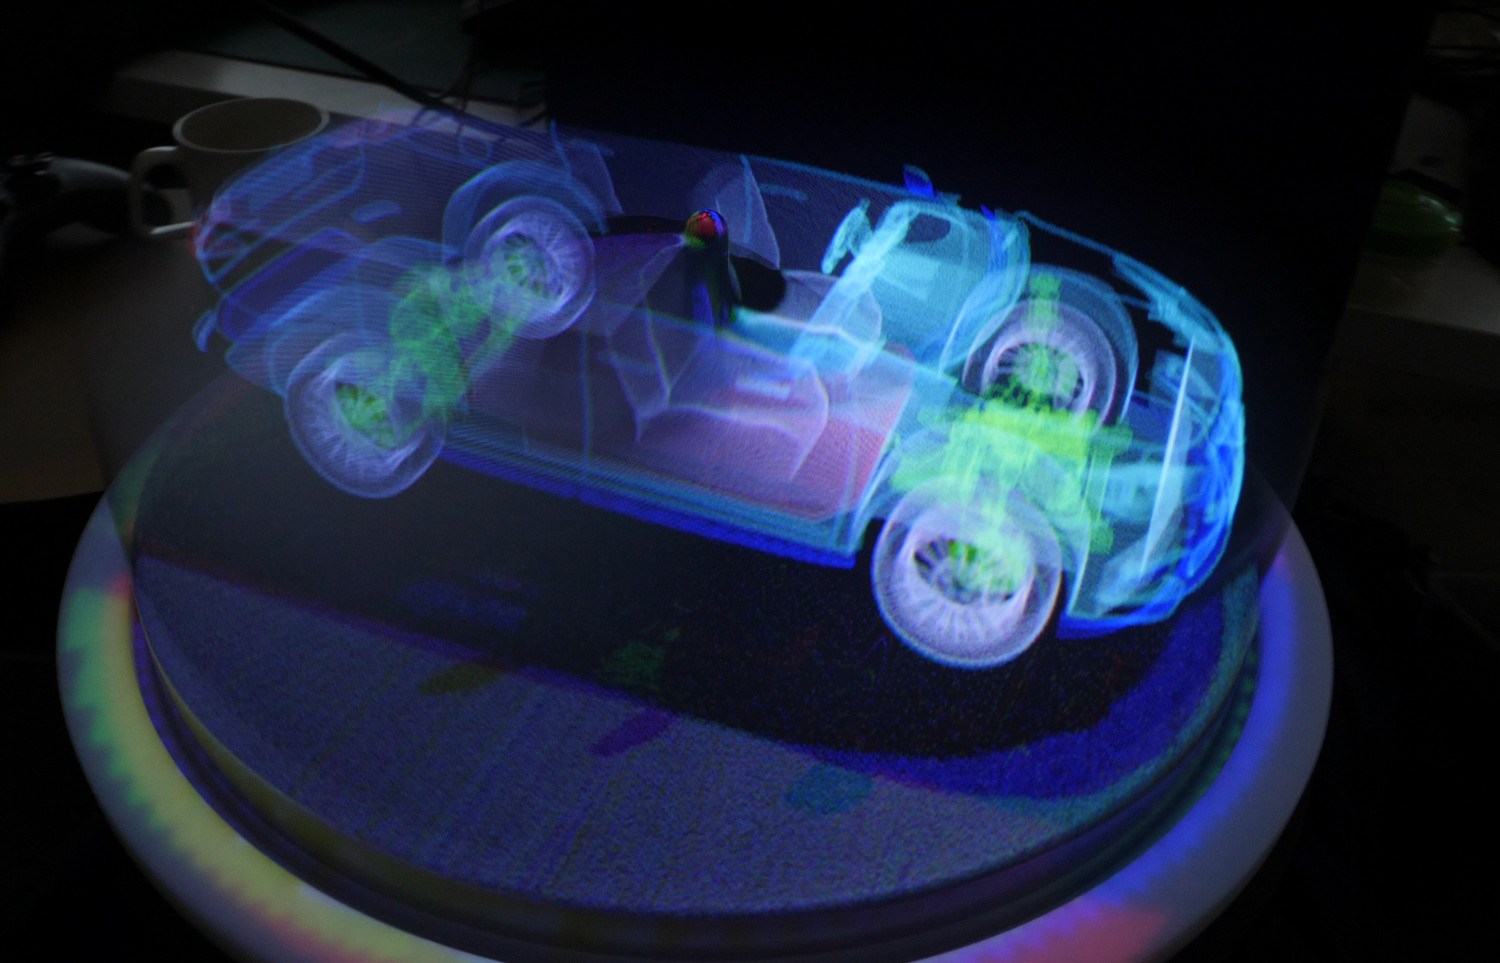
\includegraphics[width=\textwidth]{./figures/background/3d/voxon.jpg}
      \small {a) The VXR4612 3D Volumetric Display, a projector based persistence of vision display produced by Voxon Photonics.} 
    \end{minipage}\hfill
    \begin{minipage}[t]{0.48\textwidth}
      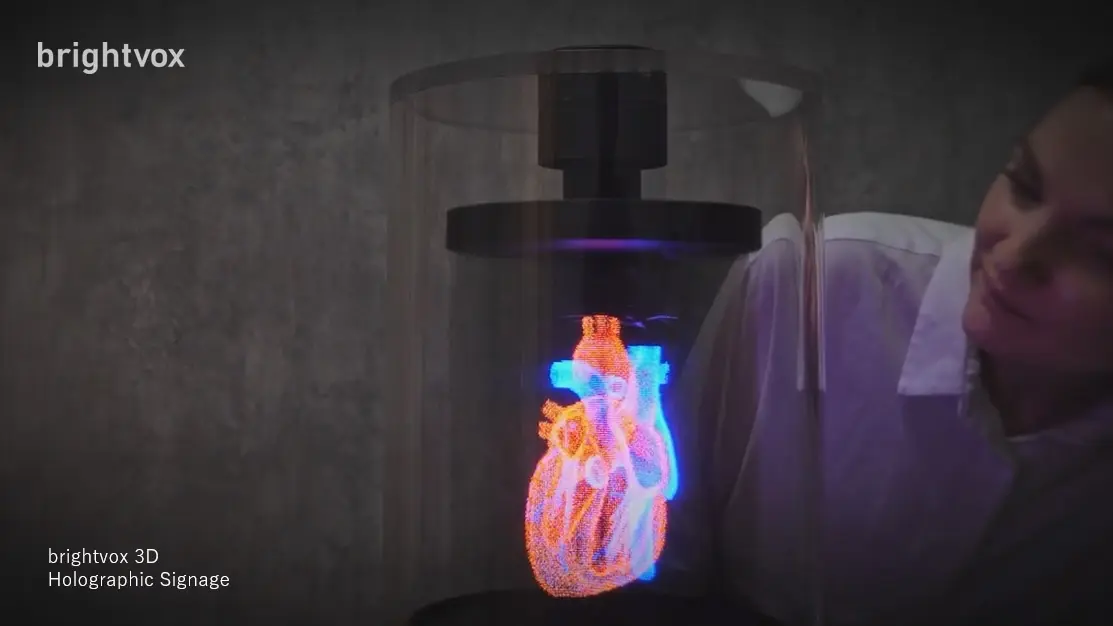
\includegraphics[width=\textwidth]{./figures/background/3d/brightvox.png}
      \small {b) A Volumetric Display / Holographic Signage, a LED based persistence of vision display produced by Brightvox Inc.}
    \end{minipage}
  \end{figureBox}
  

\subsubsection{Static Volume Displays}
Static volume displays are another category of volumetric displays. They employ a static 3D display to create a 3D image. This is achieved by emitting light from the display at each point in a 3D space. Common techniques for achieving this includes using a 3D array of LEDs, lasers, or a transparent medium that can be projected onto. Because they do not reuse the same 2D display, static volume displays are often lower resolution than swept volume displays. However, they are also more versatile, as they can be used to display a wider range of 3D objects.